% !TEX TS-program = LuaLaTeX
% !TEX encoding = UTF-8 Unicode 
% !TEX root = ../../mal-core.tex

\def\Manim{Manim}
\let\typ=\texttt
\def\maltikz{Ti\emph{k}Z}
\fboxrule=1pt
\fboxsep=0pt
\newdimen\maldelka 
\def\tecka{\includegraphics[width=3mm]{tecka.png}}
\def\tecky{\noindent\hfil\tecka\ \tecka\ \tecka}


\gdef\mujnazevCS{První kontakt s~programem \Manim}
\gdef\mujnazevEN{The first encounter with \Manim}
\gdef\mujnazevPR{\mujnazevCS}
\gdef\mujnazevDR{\mujnazevEN}
\gdef\mujauthor{Pavel Stříž}

\bonushyper

\nazev{\mujnazevCS}

\nazev{\mujnazevEN}

\author{\mujauthor}

\Email{pavel@striz.cz}

%\Adresa{}

%\smallskip


\Abstrakt{Tento článek tvoří úvod do práce s~programem \Manim\ (matematické animace) založeném na Pythonu s~podporou \TeX u. Jedná se především o~rešerši zdrojů, tipy, triky a~řešení některých problematických partií.  Program vytváří a~spravuje Grant Sanderson alias 3blue1brown a~Ben Eater. Původně to byl soukromý projekt pomáhající jim programově vytvořit náročnější videa, nyní se jedná o~otevřený software.}
\smallskip
\KlicovaSlova{Animace, \Manim, Python, \TeX}

\Abstract{This article is an introduction to work with \Manim\ software (Mathematical Animation Engine), which is a Python-based program with support of \TeX.  The paper consists mainly of research of sources, tips, tricks and  solution to some problematic parts.  Software is being developed and maintained by Grant Sanderson alias 3blue1brown and Ben Eater.  It was initially a~private project supporting them programatically create complex videos.  Now, it's an open-source software.}
\smallskip
\KeyWords{Animation, \Manim, Python, \TeX}

\bigskip


\hfill \textit{Motto: Python se má rád, je to tam jedno \texttt{self}í za druhým!}%

\vspace*{-0.5\baselineskip}

\section{Mohou za to kvaterniony}

Někdy v~roce 2018 jsem otevřel jeden ze starých problémů, a~to jak vykreslit nekonečnou trubku, ale tak, aby se vzájemně nekřížila. Je to trochu obdoba \href{https://cs.wikipedia.org/wiki/Hilbertova_k\%C5\%99ivka}{Hilbertovy křivky} (vlevo) či tvorba bludišť, např. v~programu \href{http://www.astrolog.org/labyrnth/daedalus.htm}{Daedalus} (uprostřed). Zájemce odkazuji na \href{https://www.jwz.org/xscreensaver/}{demo} (Xubuntu 18.04, obrázek vpravo): 

\begin{lstlisting}
$ sudo apt install xscreensaver xscreensaver-gl
$ xscreensaver &
$ sleep 8; xscreensaver-command -demo 39
\end{lstlisting}

\maldelka=30mm
\noindent
\fbox{\includegraphics[height=\maldelka]{hilbert1.png}}\hfill
\fbox{\includegraphics[height=\maldelka]{daedalus-3dmaze.png}}\hfill
\fbox{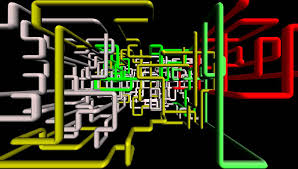
\includegraphics[height=\maldelka]{pipes1.jpeg}}%

Podařilo se mi to vyřešit v 
\href{https://www.blender.org/}{Blenderu,} ale tehdy dokumentace ke 
\href{https://cs.wikipedia.org/wiki/Kvaternion}{kvaternionům} (rozšíření komplexních čísel pro 3D) byla strohá, hledal jsem doplňující materiály. Zaujalo mě video 
\href{https://youtube.com/watch?v=d4EgbgTm0Bg}{\tt youtube.com/watch?v=d4EgbgTm0Bg} s detaily na \href{https://eater.net/quaternions}{\tt eater.net/quaternions}, ale co víc, na 
\href{https://eater.net/quaternions#comment-4164465515}{fóru} byla zmínka, že video bylo vytvořené v programu 
\href{https://github.com/3b1b/manim}{\Manim.} Tak jsem se do toho víc ponořil, neb mi název programu nic neříkal.

Zde je pár ukázek od tvůrců ze zmíněného videa:
\smallskip

\noindent
\fbox{\includegraphics[height=35.5mm]{snimek4.png}}\hfill
\fbox{\includegraphics[height=35.5mm]{snimek5.png}}%




\section{Hello World! aneb \Manim\ animuje čtverec na kolečko}

Jedná se o vyvíjený program na matematické animace a je docela programátorský oříšek dát vše do latě (instalaci, rozběhnutí ukázek, vlastní tvorba). Bral jsem to však za součást učení se.

Program lze nainstalovat přes \texttt{pip3} (\href{https://pypi.org/project/manimlib/}{\tt manimlib}), \texttt{virtualenv}, \texttt{docker}, \texttt{anaconda}, ale hlavně přímo. Detaily jsou na \href{https://github.com/3b1b/manim}{\texttt{github.com/3b1b/manim}.}

\begin{lstlisting}
$ git clone https://github.com/3b1b/manim.git
$ cd manim
$ sudo -H pip3 install -r requirements.txt
$ python3 manim.py example_scenes.py SquareToCircle -pl
\end{lstlisting}

\maldelka=21mm
\noindent
\fbox{\includegraphics[height=\maldelka]{squaretocircle0.png}}\hfill
\fbox{\includegraphics[height=\maldelka]{squaretocircle1.png}}\hfill
\fbox{\includegraphics[height=\maldelka]{squaretocircle2.png}}\hfill
\fbox{\includegraphics[height=\maldelka]{squaretocircle3.png}}\hfill
\fbox{\includegraphics[height=\maldelka]{squaretocircle4.png}}%


Pokud vše proběhne v pořádku spustí se vám video, kdy se bílý čtverec změní na barevné kolečko a to pak zmizí. 

Problém jsem měl s instalací knihovny 
\href{https://pypi.org/project/pycairo/}{\texttt{pycairo},} to jsem vůči manuálu vyřešil 
%užitím \texttt{sudo} a užitím poslední verze zásahem v \texttt{requirements.txt}. V roce 2019 jsem to vyřešil 
přes: 
\begin{lstlisting}
$ sudo apt install python3-cairo
$ sudo -H pip3 install manimlib --ignore-installed pycairo
\end{lstlisting}
%, kdy jsem \texttt{pycairo} měl již nainstalované.

Druhý řádek mi v roce 2020 nejel, stále se mi snažil vnutit \texttt{pycairo}, a~to při instalaci spadne, tak jsem užil první řádek z předchozího skriptu, v~\texttt{requirements.txt} jsem zakomentoval řádek s \texttt{pycairo} a doinstaloval jen další závislosti:
\begin{lstlisting}
$ sudo -H pip3 install -r requirements.txt 
\end{lstlisting}

Touto cestou užívám starší 
\href{https://pycairo.readthedocs.io/en/latest/}{\texttt{pycairo}} verze 1.16.2 a \Manim\ z pracovního adresáře, vše dále představené běží.



\section{Hlouběji u spuštění z příkazového řádku}

Nápovědu lze získat přes \texttt{python3 -m manim --help}. Ukázky jsou realizovány přes třídy, jejich seznam jsem si nechal vypsat přes \texttt{cat <soubor.py> | grep <třída či class>}. Obvykle vidíme 
{\tt Scene}, 
{\tt GraphScene}, 
{\tt ThreeDScene} a 
{\tt SVGMobject}.

Vytvoření videa se realizuje přes:%
\smallskip

%\begin{lstlisting}
\hfil \texttt{python3 -m manim <soubor.py> [třídy] [parametry]}%
%\end{lstlisting}
\smallskip

Třídy oddělujeme mezerami. Bez zadání třídy vyběhne nabídka a zadáváme čísla oddělená čárkou. Ne všechny třídy jsou takto spustitelné.

Nejběžnější volitelné parametry jsou následující:

\begin{itemize}
\itemsep=-2pt
\item \typ{-p} = preview, otevření souboru po dokončení,
\item \typ{-l} $|$ \typ{-m} $|$ bez parametru = velikost videa, low $|$ medium $|$ high,
\item \typ{-t} = transparent, pozadí bude průhledné,
\item \typ{-c} = color, pozadí bude mít specifickou barvu,
\item \typ{-r} = resolution, rozlišení v pixelech, výška čárka délka,
\item \typ{-s} = save the last frame, uloží z videa jen poslední snímek,
\item \typ{--livestream} $|$ \typ{--to-twitch} = živé vysílání,
\item \typ{-h} $|$ \typ{--help} = nápověda.
\end{itemize}

Výsledky se ukládají do adresáře \typ{media/video}, pak do složky dle názvu skriptu, následuje složka \typ{výška p rychlost}, např. \typ{480p15} znamená \underbar{480} \underbar{p}ixelů je výška obrazu v rychlosti \underbar{15} snímků/vteřinu. Vzniká série malých videí, které se v závěru spojí do velkého souboru mp4.

Generované \TeX ové soubory, xdv a svg lze nalézt v adresáři \typ{media/TeX}.


\section{Inspirativní zdroje}

Mezi tutoriály v angličtině řadíme 
\href{https://talkingphysics.wordpress.com/2019/01/08/getting-started-animating-with-manim-and-python-3-7/}{\url{talkingphysics.wordpress.com/2019/01/08/getting-started-animating-with-manim-and-python-3-7}} s podpůrnými soubory na 
\href{https://github.com/zimmermant/manim_tutorial}{\texttt{github.com/zimmermant/manim\_tutorial}.} Velkou inspirací jsou i zdrojové kódy na 
\href{https://github.com/Solara570/demo-solara}{\texttt{github.com/Solara570/demo-solara}.} Dal\-ší tutoriál lze nalézt na 
\href{https://github.com/malhotra5/Manim-Tutorial}{\texttt{github.com/malhotra5/Manim-Tutorial},} obsáhlý v~čínštině pak na 
\href{https://github.com/cai-hust/manim-tutorial-CN}{\texttt{github.com/cai-hust/manim-tutorial-CN}.}

Kdo dává přednost videotutoriálům, nechť nahlédne na 
\href{https://www.youtube.com/channel/UCxiWCEdx7aY88bSEUgLOC6A}{\url{youtube.com/channel/UCxiWCEdx7aY88bSEUgLOC6A}} s podpůrnými soubory na 
\href{https://github.com/Elteoremadebeethoven/AnimationsWithManim}{\url{github.com/Elteoremadebeethoven/AnimationsWithManim}.}

Za poklad ke zkoumání však lze považovat přímo ve složce \texttt{manim} adresář \texttt{from\_3b1b}, speciálně adresář \texttt{old}. Řada kódů však nejede na první dobrou, neb autoři \Manim\ přepracovávají a upravují. Nechávám otevřené pro badatele, je to spleť překlepů, programátorských háků a háčků v Pythonu.

V češtině v akad. roce 2017/2018 proběhl seminář od Mirka Olšáka, 
\url{http://www.olsak.net/mirek/manim/}, od března 2020, možná v souvislosti s~koronavirem, vznikají překlady anglických videí, 
\href{https://www.youtube.com/channel/UCIhWS2rX78OXidZ87QLkkxA}{\url{www.youtube.com/channel/UCIhWS2rX78OXidZ87QLkkxA}.}


\section{Otázky a odpovědi}

Představím některé běžné situace a jejich řešení.

\subsection{Jak řešit diakritické znaky?}

Jinými slovy, lze zasáhnout do preambule \TeX ové šablony?  Šablona je uložena v souboru \texttt{manimlib/tex\_template.tex}, po záloze souboru jsem jej upravil do této podoby:
%manimlib/utils/tex\_file\_writing.py

\lstinputlisting{zdrojaky/striz-manim/manim/manimlib/tex_template.tex}

V pozadí se užívá \texttt{latex} s převodem do svg. Přepnul jsem si na 
\href{http://luatex.org/}{\texttt{lualatex}} 
s jedním parametrem navíc v \texttt{manimlib/utils/tex\_file\_writing.py}:
%na lualatex, zakázat pdf
\begin{lstlisting}
        commands = [
            "lualatex",           # byl "latex",
            "-output-format=dvi", # přidaný řádek
\end{lstlisting}

Náš kód v souboru \texttt{ukazky/ahoj-svete.py} by mohl vypadat takto:

\noindent
\begin{minipage}{\linewidth}
\lstinputlisting{zdrojaky/striz-manim/manim/ukazky/ahoj-svete.py}
\end{minipage}

Spouštíme: \texttt{python3 -m manim ukazky/ahoj-svete.py -p}
\smallskip

\maldelka=6.7mm
\noindent
\fbox{\includegraphics[height=\maldelka]{ahojsvete0.png}}\hfill
\fbox{\includegraphics[height=\maldelka]{ahojsvete1.png}}\hfill
\fbox{\includegraphics[height=\maldelka]{ahojsvete2.png}}\hfill
\fbox{\includegraphics[height=\maldelka]{ahojsvete3.png}}%


\subsection{Lze zařadit \href{https://www.ctan.org/pkg/pgf}{\maltikz?}}
Lze, ale síla linek se v svg nebere v potaz. Chce to experimentovat u konkrétního kódu. Zde je ukázka animace pro divadelní hru v souboru \texttt{ukazky/moda-live.py}, která nebyla použita, sloužila k testovacím účelům obrazovek a~monitorů. Je vidět složitější animace, vsunutí textu do \maltikz u, u proměnných užívám \texttt{r""}, abych nemusel zdvojovat zpětná lomítka.

\lstinputlisting{zdrojaky/striz-manim/manim/ukazky/moda-live.py}

Animace: \texttt{python3 -m manim ukazky/moda-live.py -p}
\smallskip

\maldelka=18.5mm
\noindent
\fbox{\includegraphics[height=\maldelka]{modalive1.png}}\hfill
\fbox{\includegraphics[height=\maldelka]{modalive2.png}}%



\subsection{Lze animovat matematiku?}
Pozornější \TeX isté si všimli, že v preambuli šablony je balíček 
\href{https://www.ctan.org/pkg/halloweenmath}{\textsf{halloweenmath},} nyní jej použijeme v souboru \texttt{ukazky/rovnice.py}.

\lstinputlisting{zdrojaky/striz-manim/manim/ukazky/rovnice.py}

Animace: \texttt{python3 -m manim ukazky/rovnice.py -p}
\smallskip

\maldelka=9.5mm
\noindent
\fbox{\includegraphics[height=\maldelka]{rovnice1.png}}\hfill
\fbox{\includegraphics[height=\maldelka]{rovnice2.png}}\hfill
\fbox{\includegraphics[height=\maldelka]{rovnice3.png}}%


\subsection{Lze animovat kandži?}
Asi nejrychlejší způsob je si v \texttt{manimlib/constants.py} zapnout 
\href{https://ctan.org/pkg/ctex}{Chinese\TeX:}
\begin{lstlisting}
TEX_USE_CTEX = True # False
\end{lstlisting}

Tím si zajistíme, že budeme užívat 
\href{https://www.ctan.org/pkg/xetex}{\texttt{xelatex}} a \TeX ovou šablonu v souboru \texttt{manimlib/ctex\_template.tex}. Tu jsem si po odzálohování upravil do této podoby:

\noindent
\begin{minipage}{\linewidth}
\lstinputlisting{zdrojaky/striz-manim/manim/manimlib/ctex_template.tex}
\end{minipage}

\font\ipaexm=IPAexGothic at 7pt %IPAexMincho at 7pt

Jednoduchá ukázka by mohla vypadat takto:
%\lstinputlisting{zdrojaky/striz-manim/manim/ukazky/japonstina.py}

\noindent
\begin{minipage}{\linewidth}
\begin{lstlisting}[escapeinside=``]
from manimlib.imports import *
class Japonstina(Scene):
  def construct(self):
    sum1=TextMobject(r"`{\ipaexm 今日は何曜日ですか。}`")
    sum1.scale(2.5); sum1.to_edge(UP); sum1.set_color(RED); self.play(Write(sum1), run_time=3); self.wait(1)
    sum2=TextMobject(r"`{\ipaexm 3日です。}`")
    sum2.scale(6); sum2.to_edge(DOWN); sum2.set_color(RED)
    self.play(ReplacementTransform(sum1.copy(),sum2),run_time=5); self.wait(2)
\end{lstlisting}
\end{minipage}

Animaci získáme přes: \texttt{python3 -m manim ukazky/japonstina.py -p}
\smallskip

\maldelka=10mm
\noindent
\fbox{\includegraphics[height=\maldelka]{japonstina1.png}}\hfill
\smallskip

\noindent
\fbox{\includegraphics[height=\maldelka]{japonstina2.png}}\hfill
\fbox{\includegraphics[height=\maldelka]{japonstina3.png}}%


\subsection{Lze animovat výstupy z teorie grafů?}
Na pomoc jsem si vzal knihovnu \href{https://github.com/rajatvd/manimnx}{\texttt{manimnx}} a vypnul jsem si užití C\TeX u:
\begin{lstlisting}
TEX_USE_CTEX = False
\end{lstlisting}

Doinstaloval jsem si potřebné:
\begin{lstlisting}
$ git clone https://github.com/rajatvd/manimnx
$ sudo -H pip3 install networkx==2.3
\end{lstlisting}

V \texttt{manimnx/example.py} jsem zasáhl do jednoho řádku tímto způsobem, protože \texttt{manim.py} načítám z pracovního adresáře:
\begin{lstlisting}
import manimnx.manimnx.manimnx as mnx
\end{lstlisting}

Ukázka: \texttt{python3 -m manim manimnx/example.py RandomGraphs -p}
\smallskip

\maldelka=15mm
\noindent
\fbox{\includegraphics[height=\maldelka]{randomgraphs1.png}}\hfill
\fbox{\includegraphics[height=\maldelka]{randomgraphs2.png}}\hfill
\fbox{\includegraphics[height=\maldelka]{randomgraphs3.png}}\hfill
\fbox{\includegraphics[height=\maldelka]{randomgraphs4.png}}%




\subsection{Lze animovat diagramy?}
Jako poslední ukázku jsem vybral extrémní případ knihovny \href{https://github.com/graviton1221/Danim}{\texttt{Danim}.}

\begin{lstlisting}
$ git clone https://github.com/graviton1221/Danim
$ sudo -H pip3 install pandas
\end{lstlisting}

V \texttt{Danim/BubbleChart/bubblechart\_constant.py} jsem $\backslash\backslash$ upravil na /, jak pracuji pod Linuxem. A ještě jednou jsem si zapnul C\TeX.

Každý popisek se generuje do zvláštního \TeX ového souboru, vznik animace tedy trvá:
\texttt{python3 -m manim Danim/BubbleChart/BubbleChartAni} \texttt{mation.py BubbleChartAnimation -p}

Ukázka z 19. vteřiny videa v inverzních barvách kvůli tisku bulletinku.
\smallskip

\maldelka=55mm
\noindent
%\fbox{\includegraphics[height=\maldelka]{b1.png}}\hfill
\fbox{\includegraphics[width=\textwidth]{b2.png}}%
\medskip


\section{Co s programem \Manim\ neumím?}

Co jsem nepotřeboval a nezkoušel jsem do hloubky je živý přenos přes protokol tcp (parametr \texttt{--livestream}) s podporou pro Twitch přes parametry \texttt{--to-twitch} a \texttt{--with-key}. Hashovací klíč jsem našel na \href{https://www.twitch.tv/}{\tt twitch.tv} pod uživatelem; Settings; Channel and Videos a pak Primary Stream key (Copy nebo Show).

Práce se soubory svg je nativní, zde jsou oblíbené figurky přednášejících (PíCreature, Stickman a Linus). Lze si vytvořit vlastního průvodce. Nezkoušel jsem, byť návod existuje, 
\href{https://talkingphysics.wordpress.com/2018/08/14/working-with-svg-files-manim-series-part-12/}{\url{https://talkingphysics.wordpress.com/2018/08/14/working-with-svg-files-manim-series-part-12/}.}%
\smallskip

\maldelka=12.5mm
\noindent
\fbox{\includegraphics[height=\maldelka]{pi-1.png}}\hfill
\fbox{\includegraphics[height=\maldelka]{stick_man_wave.png}}\hfill
\fbox{\includegraphics[height=\maldelka]{linus.png}}\hfill
\fbox{\includegraphics[height=\maldelka]{piaci.png}}%
\smallskip

Vzniká podpora pro JavaScript, viz \href{https://github.com/JazonJiao/Manim.js}{\texttt{github.com/JazonJiao/Manim.js}.} Přes JavaScript bych na animace volil spíš \href{https://d3js.org/}{\texttt{d3js.org}.}

Vzniká též webové rozhraní, viz \href{https://github.com/eulertour/eulerv2}{\texttt{github.com/eulertour/eulerv2}.} To mi přišlo ve webovém prohlížeči extrémně pomalé.%
\medskip

\tecky\smallskip

Pokud chcete nahlédnout na animace zmíněné v článku, a programátorské a~\TeX ové věci si nezkoušet, navštivte můj skromný kanál na YouTube:
\smallskip

\noindent
\hfil\href{https://www.youtube.com/playlist?list=PLnD-4Ssyh8yOQi08n9L8WJ3wV3u2p9VO9}{\texttt{youtube.com/playlist?list=PLnD-4Ssyh8yOQi08n9L8WJ3wV3u2p9VO9}}%
\medskip

\tecky
\medskip

Co zmínit závěrem? Je to jiný svět, snad jsem vám hlavu nezamotal víc než je zdrávo, mám totiž před sebou víc otázek než odpovědí, i tak však přeji hezké bádání s nástrojem \Manim!
\begin{itemize}
\itemsep=-2pt
\item Můžeme užít \href{http://luatex.org/}{Lua\LaTeX}\ a libovolné písmo přes balíček \href{https://ctan.org/pkg/fontspec}{\textsf{fontspec}?}
\item Lze získat animaci jako sérii souborů svg?
\item Může se objekt pohybovat po libovolné křivce, např. po spirále?
\item Je možné (de)aktivovat vyhlazování písem?
\item Jak lze ideálně zařadit grafiku z programů \href{https://ctan.org/pkg/metapost}{\MP}\ a \href{https://tug.org/PSTricks/main.cgi/}{PSTricks?}
\item Jak by to bylo se zařazením 3D objektů (\href{https://asymptote.sourceforge.io/}{Asymptote}, \href{https://www.blender.org/}{Blender})?
\item Lze vložit grafické výstupy z programů typu \href{https://matplotlib.org/}{Matplotlib} a \href{https://www.r-project.org/}{R?}
\item Lze vložit do vznikající animace video? Například ve \href{https://www.youtube.com/watch?v=d4EgbgTm0Bg&feature=youtu.be&t=1467}{videu o kvaternionech} je pohyb ruky, tedy to lze, ale jak \ldots{} 
\end{itemize}

Je vidět, že 
\href{https://www.youtube.com/channel/UCYO_jab_esuFRV4b17AJtAw}{3blue1brown} 
je učitel tělem i duší a nutí nás přemýšlet a~programátorsky hledat a experimentovat. Ne nadarmo byl 13.\,3.\,2020 Grant Sanderson pozván jako řečník do TEDxBerkeley (\url{https://youtube.com/watch?v=s_L-fp8gDzY}) s tématem \textit{What Makes People Engage With Math}, minimálně jako duševní kantorská podpora v době koronaviru.%
\medskip

\hfill \emph{\ldots\ if you have a soul, you have to know why, right?}\par
\hfill --- Grant Sanderson @ \href{https://www.youtube.com/watch?v=s_L-fp8gDzY&feature=youtu.be&t=784}{00:13:04,159265}%

